%%%%%%%%%%%%%%%%%%%%%%%%%%%%%%%%%%%%%%%%%
% Beamer Presentation
% LaTeX Template
% Version 1.0 (10/11/12)
%
% This template has been downloaded from:
% http://www.LaTeXTemplates.com
%
% License:
% CC BY-NC-SA 3.0 (http://creativecommons.org/licenses/by-nc-sa/3.0/)
%
%%%%%%%%%%%%%%%%%%%%%%%%%%%%%%%%%%%%%%%%%

%----------------------------------------------------------------------------------------
%	PACKAGES AND THEMES
%----------------------------------------------------------------------------------------

\documentclass{beamer}

\mode<presentation> {

% The Beamer class comes with a number of default slide themes
% which change the colors and layouts of slides. Below this is a list
% of all the themes, uncomment each in turn to see what they look like.

%\usetheme{default}
%\usetheme{AnnArbor}
%\usetheme{Antibes}
%\usetheme{Bergen}
%\usetheme{Berkeley}
%\usetheme{Berlin}
%\usetheme{Boadilla}
%\usetheme{CambridgeUS}
%\usetheme{Copenhagen}
\usetheme{Darmstadt}
%\usetheme{Dresden}
%\usetheme{Frankfurt}
%\usetheme{Goettingen}
%\usetheme{Hannover}
%\usetheme{Ilmenau}
%\usetheme{JuanLesPins}
%\usetheme{Luebeck}
%\usetheme{Madrid}
%*\usetheme{Malmoe}
%\usetheme{Marburg}
%\usetheme{Montpellier}
%\usetheme{PaloAlto}
%\usetheme{Pittsburgh}
%\usetheme{Rochester}
%\usetheme{Singapore}
%\usetheme{Szeged}
%\usetheme{Warsaw}

% As well as themes, the Beamer class has a number of color themes
% for any slide theme. Uncomment each of these in turn to see how it
% changes the colors of your current slide theme.

%\usecolortheme{albatross}
%\usecolortheme{beaver}
%\usecolortheme{beetle}
%\usecolortheme{crane}
%\usecolortheme{dolphin}
%\usecolortheme{dove}
%\usecolortheme{fly}
%\usecolortheme{lily}
\usecolortheme{orchid}
%\usecolortheme{rose}
%\usecolortheme{seagull}
%\usecolortheme{seahorse}
%\usecolortheme{whale}
%\usecolortheme{wolverine}

%\setbeamertemplate{footline} % To remove the footer line in all slides uncomment this line
%\setbeamertemplate{footline}[page number] % To replace the footer line in all slides with a simple slide count uncomment this line

%\setbeamertemplate{navigation symbols}{} % To remove the navigation symbols from the bottom of all slides uncomment this line
}


\usepackage{graphicx} % Allows including images
\usepackage{booktabs} % Allows the use of \toprule, \midrule and \bottomrule in tables
\usepackage{xspace}
\usepackage{caption}
\usepackage{subfigure}
\usepackage[english,brazil]{babel}
\usepackage[utf8]{inputenc}

%Renomeia o nome padrao das figuras.
\renewcommand{\figurename}{Figura}
\renewcommand{\tablename}{Tabela}
%----------------------------------------------------------------------------------------
%	TITLE PAGE
%----------------------------------------------------------------------------------------

\title[Computação Gráfica]{Métodos de Rendering de Superfície} % The short title appears at the bottom of every slide, the full title is only on the title page

\author{Uéliton Freitas} % Your name
\institute[UFMS] % Your institution as it will appear on the bottom of every slide, may be shorthand to save space
{
Universidade Católica Dom Bosco - UCDB \\ % Your institution for the title page
\medskip
\textit{freitas.ueliton@gmail.com} % Your email address
}
\date{\today} % Date, can be changed to a custom date


\begin{document}

\begin{frame}
\titlepage % Print the title page as the first slide
\end{frame}

\begin{frame}
\frametitle{Sumário} % Table of contents slide, comment this block out to remove it
\tableofcontents % Throughout your presentation, if you choose to use \section{} and \subsection{} commands, these will automatically be printed on this slide as an overview of your presentation
\end{frame}




%----------------------------------------------------------------------------------------
%	PRESENTATION SLIDES
%----------------------------------------------------------------------------------------

%------------------------------------------------
\section{Introdução} 
%------------------------------------------------

%\section{Speeded-Up Robust Features - SURF} % A subsection can be created just before a set of slides with a common theme to further break down your presentation into chunks
%\section{Baf Of Features and Colors}

%\section{Refer\^encias}
%%%%%%%%%%%%%%%%%%%%%%%%%%%%%%%%%%%%%%%%%%%%%%%%%%%%%%%%%%%%%%%%%%%%%%%%%%%%%%%%%%%%%%%%%%
\begin{frame}
\frametitle{Introdução}

		\begin{block}{Introdução}
		\begin{itemize}
			\item Baseado no modelo de Iluminação, um método de \textbf{rendering de superfície} é usado para determinar a cor dos pixels.
			\item O modelo de iluminação pode ser usado de formas diferentes para definir a cor de uma superfície.
			\begin{itemize}
				\item \textbf{Ray-Tracing}: executado em cada pixel (maior realismo).
				\item \textbf{Scan-Line}: Escutado em alguns pixels e interpolado no restante(tempo real).
			\end{itemize}					 
		\end{itemize}
	\end{block}
	
\end{frame}



%%%%%%%%%%%%%%%%%%%%%%%%%%%%%%%%%%%%%%%%%%%%%%%%%%%%%%%%%%%%%%%%%%%%%%%%%%%%%%%%%%%%%%%%%%
\begin{frame}
\frametitle{Introdução}

		\begin{block}{Introdução}
		\begin{itemize}
			\item A maioria das API's gráficas reduz  o processamento usando scan-line.
			\begin{itemize}
				\item As intensidades são calculadas em cada vértice e interpoladas nas regiões restantes dos polígonos.
			\end{itemize}							 
		\end{itemize}
	\end{block}
	
\end{frame}

%%%%%%%%%%%%%%%%%%%%%%%%%%%%%%%%%%%%%%%%%%%%%%%%%%%%%%%%%%%%%%%%%%%%%%%%%%%%%%%%%%%%%%%%%%
\section{Rendering de Superfícies com Intensidade Constante}
\begin{frame}
\frametitle{Rendering de Superfícies com Intensidade Constante}

		\begin{block}{Rendering de Superfícies com Intensidade Constante}
		\begin{itemize}
			\item O método mais simples para renderizar uma superfície é usar a mesma cor para todos os seus piexel (\textbf{flat Surface rendering}).
			\item O modelo de iluminação é empregado para determinar a intensidade das 3 componentes RGB em uma única posição da superfície.
			\begin{itemize}
				\item Vértice ou centroide do polígono.
			\end{itemize}						 
		\end{itemize}
	\end{block}
	
		\begin{figure}[!h]
			\begin{center}
			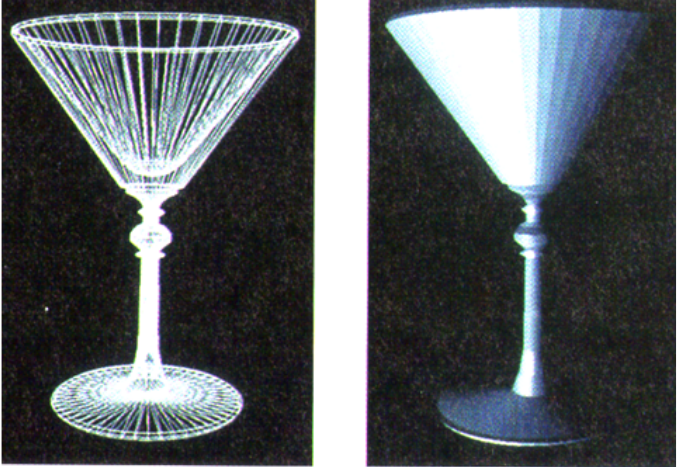
\includegraphics[width=0.4\textwidth]{Figures/FlaSur}
			\end{center}
		\end{figure}
	
\end{frame}

%%%%%%%%%%%%%%%%%%%%%%%%%%%%%%%%%%%%%%%%%%%%%%%%%%%%%%%%%%%%%%%%%%%%%%%%%%%%%%%%%%%%%%%%%%
\begin{frame}
\frametitle{Rendering de Superfícies com Intensidade Constante}

		\begin{block}{Rendering de Superfícies com Intensidade Constante}
		\begin{itemize}
			\item A \textbf{flat surface rendering} possui bons resultados quando:
			\begin{itemize}
				\item O polígono é uma face de um pliedro e \textbf{não} uma uma seção de uma \textbf{superfície curva}.
				\item Todas as \textbf{fontes de luz} estão \textbf{longe o suficiente} da superfície de forma que $\textbf{N} \cdot \textbf{L}$ e a função de atenuação são \textbf{constantes} 
				\item A \textbf{posição de visão} é \textbf{distante} o suficiente do polígono de forma que $\textbf{V} \cdot \textbf{R}$(ou $\textbf{N} \cdot \textbf{H}$) é constante.\\
				\begin{equation*}
					I=k_aI_a + \sum_{l=1}^n I_l[k_d(\textbf{N} \cdot \textbf{L}) +k_s(\textbf{N}\cdot \textbf{H})^{ns}]
				\end{equation*}
				\item Mesmo se uma das condições for falsa, uma boa aproximação pode ser feita se os polígonos forem pequenos.
			\end{itemize}
		\end{itemize}
	\end{block}
	
\end{frame}


%%%%%%%%%%%%%%%%%%%%%%%%%%%%%%%%%%%%%%%%%%%%%%%%%%%%%%%%%%%%%%%%%%%%%%%%%%%%%%%%%%%%%%%%%%
\section{Rendering de Superfícies de Gouraud}
\begin{frame}
\frametitle{Rendering de Superfícies de Gouraud}

		\begin{block}{Rendering de Superfícies de Gouraud}
		\begin{itemize}
			\item O rendering de superfície de Gouraud interpola linearmente as intensidades nos vértices por toda a face do polígono de um objeto iluminado.
			\item Foi desenvolvido para aproximar superfícies curvas e amenizar as transições de intensidades entre polígonos adjacentes.
			\begin{itemize}
				\item Elimina a descontinuidade de intensidades de cor da \textbf{flat surface rendering}.
			\end{itemize}
		\end{itemize}
	\end{block}
	
\end{frame}

%%%%%%%%%%%%%%%%%%%%%%%%%%%%%%%%%%%%%%%%%%%%%%%%%%%%%%%%%%%%%%%%%%%%%%%%%%%%%%%%%%%%%%%%%%
\begin{frame}
\frametitle{Rendering de Superfícies de Gouraud}

		\begin{block}{Rendering de Superfícies de Gouraud}
		\begin{itemize}
			\item Cada polígono de uma superfície é processado usando os seguintes métodos:
			\begin{enumerate}
				\item Determina-se o vetor unitário normal médio em cada vértice do polígono.
				\item Aplica-se o modelo de iluminação em cada vértice para obter as intensidades.
				\item Interpola linearmente as intensidades dos vértices sobre a área projetada do polígono.
			\end{enumerate}
		\end{itemize}
	\end{block}
	
\end{frame}


%%%%%%%%%%%%%%%%%%%%%%%%%%%%%%%%%%%%%%%%%%%%%%%%%%%%%%%%%%%%%%%%%%%%%%%%%%%%%%%%%%%%%%%%%%
\begin{frame}
\frametitle{Rendering de Superfícies de Gouraud}

		\begin{block}{Rendering de Superfícies de Gouraud}
		\begin{itemize}
			\item O vetor normal médio \textbf{N} em um vértice é obtido fazendo a média das normais de todos os polígonos que compartilham esse vértice.
			\begin{equation*}
				\textbf{N}_v = \frac{\sum_{k=1}^n \textbf{N}_k}{|\sum_{k=1}^n \textbf{N}_k|}
			\end{equation*}
			\item Usando essas normais o modelo de iluminação é aplicado e então executado para calcular as intensidades de cada vértice.
		\end{itemize}
	\end{block}
	
	\begin{figure}[!h]
			\begin{center}
			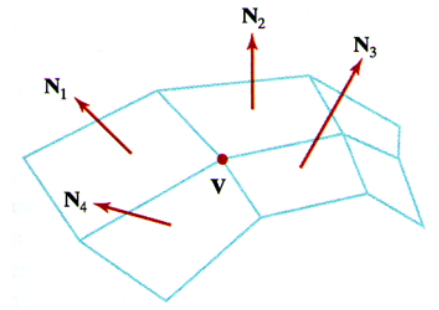
\includegraphics[width=0.4\textwidth]{Figures/NorMea}
			\end{center}
		\end{figure}
	
\end{frame}

%%%%%%%%%%%%%%%%%%%%%%%%%%%%%%%%%%%%%%%%%%%%%%%%%%%%%%%%%%%%%%%%%%%%%%%%%%%%%%%%%%%%%%%%%%
\begin{frame}
\frametitle{Rendering de Superfícies de Gouraud}

		\begin{block}{Rendering de Superfícies de Gouraud}
		\begin{itemize}
			\item Estes valores de intensidade são então interpolados para se obter as intensidades ao longo de \textbf{scan-lines} que intersectam a área projetada do polígono.
			\item As intensidades das intersecções das scan-lines com as arestas dos polígonos são calculadas interpolando linearmente as intensidades dos pontos finais das retas. 
		\end{itemize}
	\end{block}
	
	\begin{figure}[!h]
			\begin{center}
			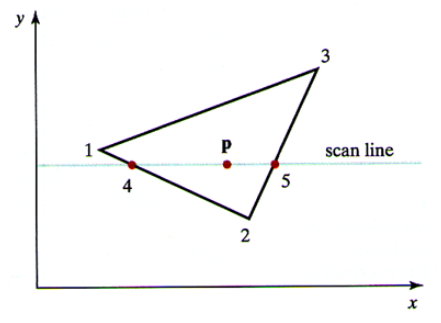
\includegraphics[width=0.4\textwidth]{Figures/Int1}
			\end{center}
		\end{figure}
	
\end{frame}


%%%%%%%%%%%%%%%%%%%%%%%%%%%%%%%%%%%%%%%%%%%%%%%%%%%%%%%%%%%%%%%%%%%%%%%%%%%%%%%%%%%%%%%%%%
\begin{frame}
\frametitle{Rendering de Superfícies de Gouraud}

		\begin{block}{Rendering de Superfícies de Gouraud}
		\begin{itemize}
			\item Por exemplo, a intensidade em 4 pode ser obtida considerando somente os deslocamento vertical da scan-line.
			\begin{equation*}
				I_4 = \frac{y_4-y_2}{y_1-y_2} I_1 + \frac{y_1-y_4}{y_1-y_2}I_2
			\end{equation*}
			\item A intensidade de 5 é obtida de forma análoga.
			\end{itemize}
	\end{block}
	
	\begin{figure}[!h]
			\begin{center}
			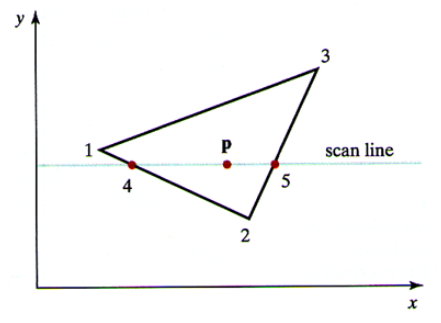
\includegraphics[width=0.4\textwidth]{Figures/Int1}
			\end{center}
		\end{figure}
	
\end{frame}


%%%%%%%%%%%%%%%%%%%%%%%%%%%%%%%%%%%%%%%%%%%%%%%%%%%%%%%%%%%%%%%%%%%%%%%%%%%%%%%%%%%%%%%%%%
\begin{frame}
\frametitle{Rendering de Superfícies de Gouraud}

		\begin{block}{Rendering de Superfícies de Gouraud}
		\begin{itemize}
			\item Considerando as intensidades obtidas em 4 e 5, as intensidades de qualquer ponto \textbf{p} sobre a scan-line são obtidas interpoladas na horizontal. 
			\begin{equation*}
				I_4 = \frac{x_5-x_p}{x_5-x_4} I_4 + \frac{x_p-x_1}{x_5-x_4}I_5
			\end{equation*}
			\item Este método é conhecido como interpolação \textbf{bilinear} e é executado para os 3 componentes RGB separadamente.
			\end{itemize}
	\end{block}
	
	\begin{figure}[!h]
			\begin{center}
			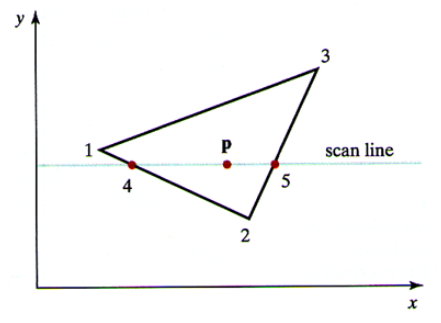
\includegraphics[width=0.3\textwidth]{Figures/Int1}
			\end{center}
		\end{figure}
	
\end{frame}

%%%%%%%%%%%%%%%%%%%%%%%%%%%%%%%%%%%%%%%%%%%%%%%%%%%%%%%%%%%%%%%%%%%%%%%%%%%%%%%%%%%%%%%%%%
\begin{frame}
\frametitle{Rendering de Superfícies de Gouraud}

		\begin{block}{Rendering de Superfícies de Gouraud}
		\begin{itemize}
			\item Esta interpolação de intensidades elimina descontinuidades mas ainda assim há alguns \textbf{problemas}.
			\begin{itemize}
				\item Brilhos na superfície podem apresentar formatos estranhos.
				\item Intensidades claras ou escuras podem parecer ``riscadas''(\textbf{mach bands}).
			\end{itemize}
			\end{itemize}
	\end{block}
	
	\begin{figure}[!h]
			\begin{center}
			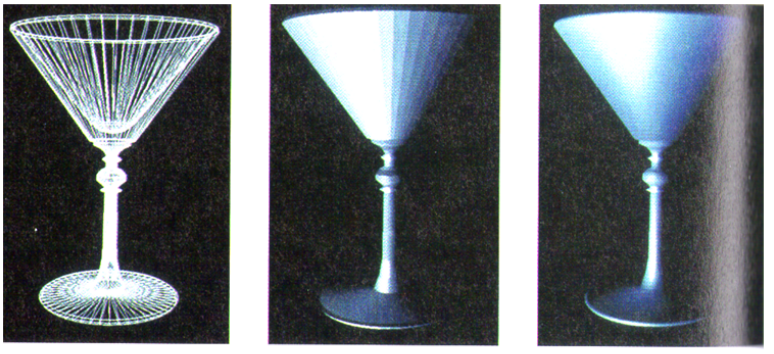
\includegraphics[width=0.7\textwidth]{Figures/MatBan}
			\end{center}
		\end{figure}
\end{frame}


%%%%%%%%%%%%%%%%%%%%%%%%%%%%%%%%%%%%%%%%%%%%%%%%%%%%%%%%%%%%%%%%%%%%%%%%%%%%%%%%%%%%%%%%%%
\begin{frame}
\frametitle{Rendering de Superfícies de Gouraud}

		\begin{block}{Rendering de Superfícies de Gouraud}
		\begin{itemize}
			\item Efeitos de \textbf{match bands} consiste em faixas claras ou escuras que são percebidas próximo das fronteiras entre duas regiões de diferentes gradientes de luz.
		\end{itemize}
	\end{block}
	
	\begin{figure}[!h]
			\begin{center}
			
\includegraphics[width=0.7\textwidth]{Figures/graCor}
			\end{center}
		\end{figure}
\end{frame}


%%%%%%%%%%%%%%%%%%%%%%%%%%%%%%%%%%%%%%%%%%%%%%%%%%%%%%%%%%%%%%%%%%%%%%%%%%%%%%%%%%%%%%%%%%
\section{Rendering de Superfícies de Phong}
\begin{frame}
\frametitle{Rendering de Superfícies de Phong}

		\begin{block}{Rendering de Superfícies de Phong}
		\begin{itemize}
			\item Um método mais preciso de interpolação é conhecido como \textbf{Phong surface rendering}.
			\item Ao invés de interpolar valores de intensidades, normais são interpoladas.
			\begin{itemize}
				\item Cálculos mais precisos de intensidades.
				\item Brilhos mais realísticos de superfícies.
				\item Redução do feitos match-band.
			\end{itemize}
			\item Contudo é mais custoso computacionalmente do que o método de Gouraud.
		\end{itemize}
	\end{block}
\end{frame}

%%%%%%%%%%%%%%%%%%%%%%%%%%%%%%%%%%%%%%%%%%%%%%%%%%%%%%%%%%%%%%%%%%%%%%%%%%%%%%%%%%%%%%%%%%
\begin{frame}
\frametitle{Rendering de Superfícies de Phong}

		\begin{block}{Rendering de Superfícies de Phong}
		\begin{itemize}
			\item Cada polígono é processado da seguinte forma:
			\begin{enumerate}
				\item Determina-se o vetor unitário médio de cada vértice do polígono.
				\item Interpola-se linearmente as normais dos vértices sobre a área projetada do polígono.
				\item Aplica-se o modelo de iluminação nas posições ao longo da scan-line para calcular a intensidade dos pixels usando as normais interpoladas.
			\end{enumerate}
		\end{itemize}
	\end{block}
\end{frame}

%%%%%%%%%%%%%%%%%%%%%%%%%%%%%%%%%%%%%%%%%%%%%%%%%%%%%%%%%%%%%%%%%%%%%%%%%%%%%%%%%%%%%%%%%%
\begin{frame}
\frametitle{Rendering de Superfícies de Phong}

		\begin{block}{Rendering de Superfícies de Phong}
		\begin{itemize}
			\item O procedimento de interpolação das normais é o mesmo da interpolação das intensidades do método de Gouraud.
			\item Por exemplo, o vetor \textbf{N} é verticalmente interpolado a partir das normais nos vértices 1 e 2 da seguinte forma:
			\begin{equation*}
				\textbf{N} = \frac{y-y_2}{y_1-y_2}\textbf{N}_1+\frac{y_1-y}{y_1-y_2}\textbf{N}_2
			\end{equation*}
		\end{itemize}
	\end{block}
	
		\begin{figure}[!h]
			\begin{center}
			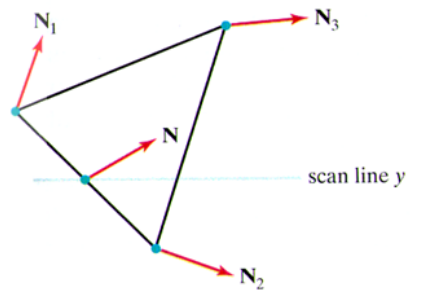
\includegraphics[width=0.4\textwidth]{Figures/IntPho}
			\end{center}
		\end{figure}
\end{frame}



%----------------------------------------------------------------------------------------
\end{document} 